% !TEX root = Projektdokumentation.tex
\section{Anhang}
% !TEX root = ../Diplombericht.tex
\section{Vorbereitungen RPI's}
\subsection{Betriebssystem installieren}
Für die Installation des CentOS 7.4 ist kein boot fähiger Kernel vorhanden. Das RPI kann aber dennoch mit einem Centos 7.4 betrieben werden. Dafür sind die folgenden Schritte vorzunehmen. Die Installation des Betriebssystems ist von einem Fedora Linux Client aus beschrieben.

1. Gentoo 64 Bit Image herunterladen aus dem Github Repository\footnote{\url{https://github.com/sakaki-/gentoo-on-rpi3-64bit}} von Sakaki\newline
2. Das Archiv wird mit dem Fedora Media Writer auf die SD Karte geschrieben. Dies ist anhand der Screenshots beschrieben. \newline
\begin{figure}[H]
	\centering
	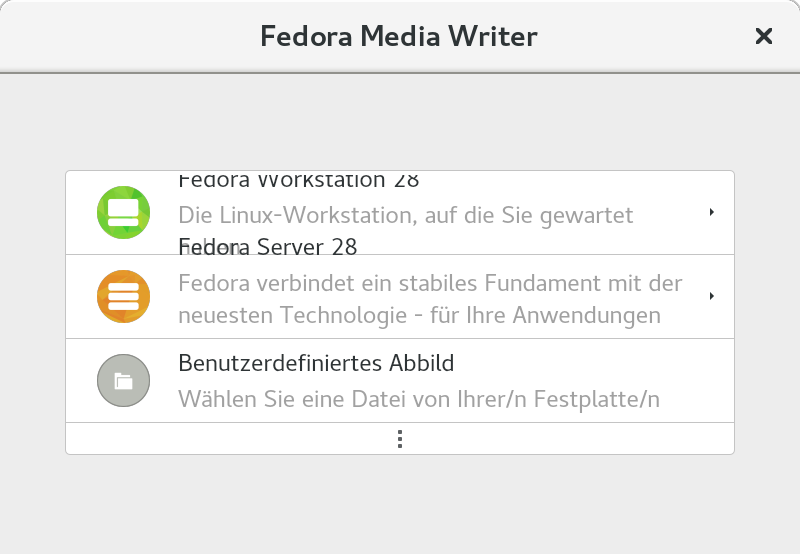
\includegraphics[scale=0.3]{Bilder/fmw1.png}
	\caption{FMW: Fedora Media Writer starten}
\end{figure}
\begin{figure}[H]
	\centering
	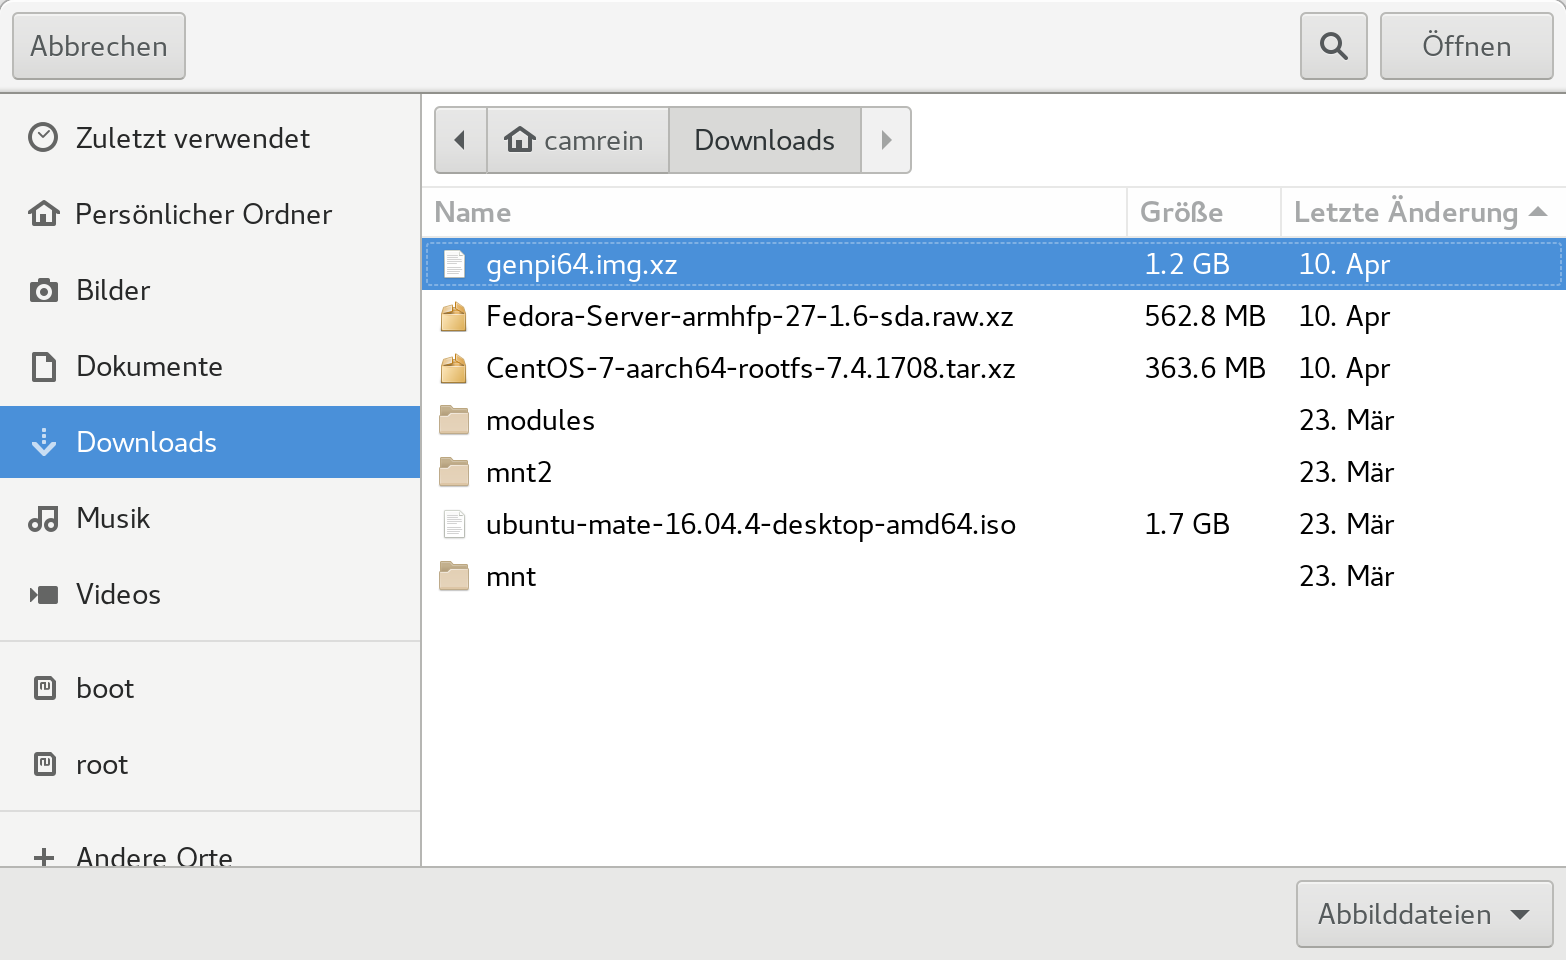
\includegraphics[scale=0.2]{Bilder/fmw2.png}
	\caption{FMW: Archiv auswählen}
\end{figure}
\begin{figure}[H]
	\centering
	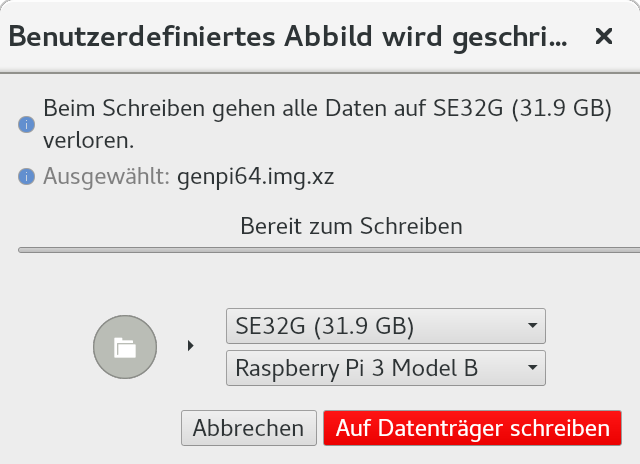
\includegraphics[scale=0.3]{Bilder/fmw3.png}
	\caption{FMW: Abbild schreiben}
\end{figure}
3. Durch das Schreiben des Archivs wurden zwei Partitionen (boot \& rootfs) auf der SD Karte erstellt. Diese werden wie folgt ausgelesen:
\begin{lstlisting}
[camrein@wifibridge ~]\$ lsblk
NAME MAJ:MIN RM SIZE RO TYPE MOUNTPOINT
sda 8:0 0 238.5G 0 disk 
-sda1 8:1 0 200M 0 part /boot/efi
-sda2 8:2 0 1G 0 part /boot
-sda3 8:3 0 237.3G 0 part 
--fedora-root 253:0 0 50G 0 lvm /
--fedora-swap 253:1 0 7.8G 0 lvm [SWAP]
--fedora-home 253:2 0 179.5G 0 lvm /home
mmcblk0 179:0 0 29.7G 0 disk}
-mmcblk0p1 179:1 0 43.1M 0 part /run/media/camrein/boot
-mmcblk0p2 179:2 0 29.7G 0 part /run/media/camrein/rootfs
[camrein@wifibridge ~]\$
\end{lstlisting}
4. Die Dateisystem-Partition muss mit der von CentOS überschrieben werden. Dazu wird die Partition auf dem Linux Client angehängt. Bei Schritt 5-7 wird überprüft, ob die Partition wirklich leer ist.
\begin{lstlisting}
[root@wifibridge Downloads]# mkdir mnt
[root@wifibridge Downloads]# mount /dev/mmcblk0p2 mnt
[root@wifibridge Downloads]# cd mnt
[root@wifibridge mnt]# rm -rf *
[root@wifibridge mnt]# ls -lrtha
drwxr-xr-x. 5 camrein camrein 20K 15. Mai 17:39 ..
drwxr-xr-x. 2 root root 4.0K 16. Mai 17:58 .
\end{lstlisting}

Die Dateisystem-Partition ist nun leer und kann mit der von CentOS überschrieben werden. \newline
5. Das Dateisystem aus dem offiziellen Centos Repository\footnote{\url{http://mirror.centos.org/altarch/7.4.1708/isos/aarch64/CentOS-7-aarch64-rootfs-7.4.1708.tar.xz}} beziehen. \newline
6. Die geleerte Partition wird nun mit dem Dateisystem von Centos7.4 überschrieben. Zugleich soll bei Schritt 2 überprüft werden, ob die Daten wirklich auf die Partition geschrieben wurden.
\begin{lstlisting}
[root@wifibridge mnt]# tar --numeric-owner -xpJf ../CentOS-7-aarch64-rootfs-7.4.1708.tar.xz
[root@wifibridge mnt]# ls -lrtha
insgesamt 84K
drwxr-xr-x. 2 root root 4.0K 23. Nov 2016 srv
drwxr-xr-x. 2 root root 4.0K 23. Nov 2016 opt
drwxr-xr-x. 2 root root 4.0K 23. Nov 2016 mnt
drwxr-xr-x. 2 root root 4.0K 23. Nov 2016 media
drwxr-xr-x. 2 root root 4.0K 23. Nov 2016 home
drwxr-xr-x. 2 root root 4.0K 12. Sep 2017 dev
drwxr-xr-x. 2 root root 4.0K 12. Sep 2017 proc
drwxr-xr-x. 2 root root 4.0K 12. Sep 2017 run
drwxr-xr-x. 2 root root 4.0K 12. Sep 2017 sys
lrwxrwxrwx. 1 root root 7 12. Sep 2017 bin -> usr/bin
lrwxrwxrwx. 1 root root 8 12. Sep 2017 sbin -> usr/sbin
lrwxrwxrwx. 1 root root 9 12. Sep 2017 lib64 -> usr/lib64
lrwxrwxrwx. 1 root root 7 12. Sep 2017 lib -> usr/lib
drwxr-xr-x. 13 root root 4.0K 12. Sep 2017 usr
drwxr-xr-x. 19 root root 4.0K 12. Sep 2017 var
dr-xr-xr-x. 17 root root 4.0K 12. Sep 2017 .
drwxr-xr-x. 82 root root 4.0K 12. Sep 2017 etc
dr-xr-xr-x. 3 root root 4.0K 12. Sep 2017 boot
drwxrwxrwt. 7 root root 4.0K 12. Sep 2017 tmp
dr-xr-x---. 2 root root 4.0K 12. Sep 2017 root
drwxr-xr-x. 5 camrein camrein 20K 15. Mai 17:39 ..
[root@wifibridge mnt]#
\end{lstlisting}

Die SD Karte kann nun mit den RPI's verwendet werden. Diese starten jeweils mit dem Hostnamen centos.


\subsection{RPI für den Netzwerkboot vorbereiten}
Für das Vorbereiten der Clients für den Netzwerkboot wurde der Guide NETWORK BOOT YOUR RASPBERRY PI von raspberrypi.org\footnote{\url{https://www.raspberrypi.org/documentation/hardware/raspberrypi/bootmodes/net\_tutorial.md}} verwendet. Die RPI's werden wie folgt vorbereitet:

1. Die config.txt Datei im /boot Verzeichnis benötigt einen OTP Eintrag, dieser sagt aus, dass das RPI ohne SD Karte nach einem Betriebssystem anfragen soll. 
\begin{lstlisting}
echo program_usb_boot_mode=1 | sudo tee -a /boot/config.txt
\end{lstlisting}
2. RPI neu starten. \newline
3. Prüfen, ob die Änderung aktiv ist.
\begin{lstlisting}
vcgencmd otp_dump | grep 17:
\end{lstlisting}
Erwartetes Ergebnis:
\begin{lstlisting}
17:3020000a
\end{lstlisting}
4. Den Eintrag in der /boot/config.txt wieder entfernen.\newline
\textbf{MAC-Adressen auslesen}\newline
Um Zeit zu sparen können alle MAC-Adressen der RPI's während der Vorbereitung der Clients auf den Netzwerkboot ausgelesen werden.\newline
5. nmap Scan auf die IP Range 192.168.1.0-255 von einem Linux Client aus durchführen.
\begin{lstlisting}
	  nmap -sP 192.168.1.0/24  
\end{lstlisting}
Erwartetes Ergebnis für ein RPI:
\begin{lstlisting}
	  Nmap scan report for centos.home (192.168.1.11)
	  Host is up (0.00055s latency).
	  MAC Address: B8:27:EB:32:39:A7 (Raspberry Pi Foundation)   
\end{lstlisting}

Die Vorbereitung der RPI(Compute Nodes) ist somit abgeschlossen und es kann mit der Installation des Management Node fortgefahren werden.

\subsection{Hostname und IP der MAC Adresse zuweisen}
über http://internetbox/ wird die IP Adresse sowie der Hostname der MAC Adresse der RPI's zugewiesen. Alle jemals angeschlossenen Geräte werden unter der Geräteliste aufgelistet. Dort können ebenfalls die Hostnamen den Geräten zugewiesen werden.

\begin{figure}[H]
	\centering
	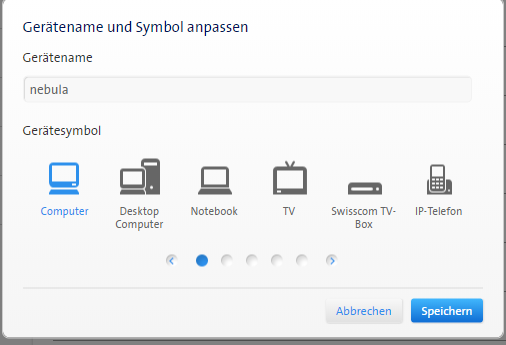
\includegraphics[scale=0.8]{Bilder/hostnamen_mac_edit.png}
	\caption{Hostnamen editieren}
\end{figure}
\begin{figure}[H]
	\centering
	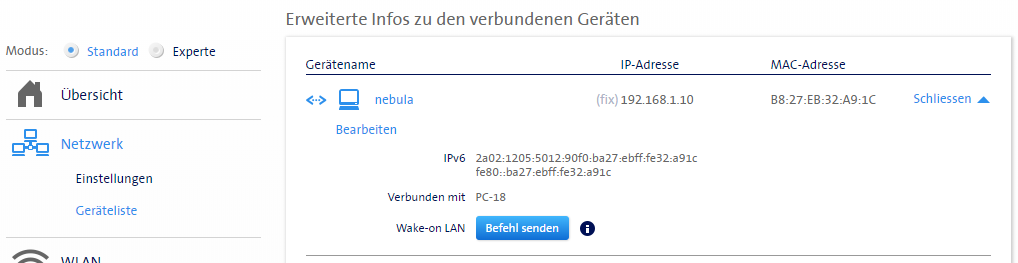
\includegraphics[scale=0.6]{Bilder/hostnamen_mac_overview.png}
	\caption{Übersicht der Hostnamen Zuweisung}
\end{figure}

Die fixe IP Adresse wird unter den Netzwerkeinstellungen des Routers direkt vorgenommen. Hierbei kann den bereits erkannten und definierten RPI's per Hostname eine IP zugewiesen werden.
\begin{figure}[H]
	\centering
	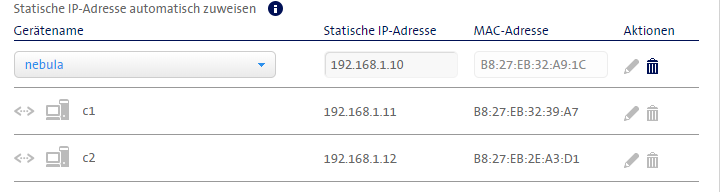
\includegraphics[scale=0.8]{Bilder/ip_mac_edit.png}
	\caption{Statische IP vergeben}
\end{figure}

\subsection{Netzwerkshare einrichten}
Der Netzwerkshare wird über das Synology NAS mit dem Network File System (NFS) Protkoll bereitgestellt. Der Share wird gemäss den aufgelisteten Schritten erstellt. \newline

1. Über den Browser auf das NAS via http://influbox/ verbinden. \newline
2. Anmeldedaten eingeben. \newline
3. Über die Systemsteuerung die Einstellungen für Dateidienste aufrufen. \newline
4. Unter dem Reiter SMB/AFP/NFS soll die Funktion \grqq NFS aktivieren\grqq aktiviert werden. \newline
5. Der NFS Dienst ist nun aktiviert und es kann unter \grqq Gemeinsam Ordner\grqq ein neues Verzeichnis angelegt werden. Dieses Verzeichnis wird der Mountpoint für die Nodes. Der Mountpoint wurde nebula genannt. \newline
6. Für den erstellten Ordner müssen nun noch die Berechtigungen für Zugriffe eingerichtet werden. Dazu bearbeitet man unter Einstellungen die Rechte auf das Verzeichnis. \newline
7. Damit nicht jeder das Verzeichnis mounten kann, wurde  auf 192.168.10/24  eingegrenzt. Dies kann über das GUI von Synology direkt eingerichtet werden.
\begin{figure}[H]
	\centering
	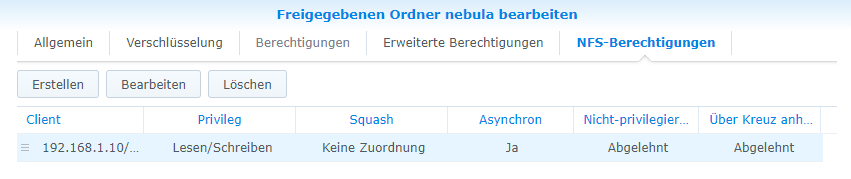
\includegraphics[scale=0.8]{Bilder/nfs_net.png}
	\caption{NFS: Erlaubte Clients}
\end{figure}
8. Der Netzwerkshare kann von nun an auf dem Management Node und den Computes eingebunden werden.
% !TEX root = ../Diplombericht.tex

\section{Installation Management Node}
Die Serverinstallation des Management Nodes wird nach dem offiziellen OpenHPC Guide mit einigen Abweichungen durchgeführt. Die Installation basiert auf der Anleitung CentOS 7.4 aarch64 Install guide with Warewulf + Slurm \footnote{\url{http://openhpc.community/downloads/}}. Die Installation wird hauptsächlich mit dem ROOT-Benutzer durchgeführt, falls nichts anderes erwähnt wird.

\subsection{Variablen Definition}
Durch die Installation hinweg werden die folgenden Variablen verwendet:

\begin{longtable}{| p{0.5cm} | p{3cm} | p{8.5cm} | p{4cm} |} 
\hline
\rowcolor{heading} \textbf{Nr.} & \textbf{Variable} & \textbf{Beschreibung} &\textbf{Werte} \\\hline
1 & sms\_name & Hostname des Managementhosts & nebula \\\hline
2 & sms\_ip & IP Adresse des Managementhosts & 192.168.1.10 \\\hline
3 & sms\_eth\_internal & Ethernet Interface & eth0 \\\hline
4 & ntp\_server[0] \newline ntp\_server[1] \newline ntp\_server[2] \newline ntp\_server[3] & Zeitserver (Array) & server 0.ch.pool.ntp.org \newline server 1.ch.pool.ntp.org \newline server 2.ch.pool.ntp.org \newline server 3.ch.pool.ntp.org  \\\hline
5 & num\_computes & Anzahl Compute Nodes & 45 \\\hline
6 &  c\_ip[0] \newline  c\_ip[1] \newline c\_ip[2] \newline c\_ip[3] \newline c\_ip[4] \newline c\_ip[5] \newline c\_ip[6] \newline c\_ip[7] \newline c\_ip[8] \newline c\_ip[9] \newline c\_ip[10] \newline c\_ip[11] \newline c\_ip[12] \newline c\_ip[13] \newline c\_ip[14] \newline c\_ip[15] \newline c\_ip[16] \newline c\_ip[17] \newline c\_ip[18] & IP Adressen der Compute Nodes (Array) & 192.168.1.11 \newline 192.168.1.12 \newline 192.168.1.13 \newline 192.168.1.14 \newline 192.168.1.15 \newline 192.168.1.16 \newline 192.168.1.17 \newline 192.168.1.18 \newline 192.168.1.19 \newline 192.168.1.20 \newline 192.168.1.21 \newline 192.168.1.22 \newline 192.168.1.23 \newline 192.168.1.24 \newline 192.168.1.25 \newline 192.168.1.26 \newline 192.168.1.27 \newline 192.168.1.28 \newline 192.168.1.29 \\\hline 
\rowcolor{heading} \textbf{Nr.} & \textbf{Variable} & \textbf{Beschreibung} &\textbf{Werte} \\\hline
6 & c\_ip[19] \newline c\_ip[20] \newline c\_ip[21] \newline c\_ip[22] \newline c\_ip[23] \newline c\_ip[24]  \newline c\_ip[25] \newline c\_ip[26] \newline c\_ip[27] \newline c\_ip[28] \newline c\_ip[29]  \newline c\_ip[30] \newline c\_ip[31] \newline c\_ip[32] \newline c\_ip[33] \newline c\_ip[34] \newline c\_ip[35] \newline c\_ip[36] \newline c\_ip[37] \newline c\_ip[38] \newline c\_ip[39] \newline c\_ip[40] \newline c\_ip[41] \newline c\_ip[42] \newline c\_ip[43] \newline c\_ip[44] & IP Adressen der Compute Nodes (Array) &  192.168.1.30 \newline 192.168.1.31 \newline 192.168.1.32 \newline  192.168.1.33 \newline 192.168.1.34 \newline 192.168.1.35 \newline 192.168.1.36 \newline 192.168.1.37 \newline 192.168.1.38 \newline 192.168.1.39 \newline 192.168.1.40 \newline 192.168.1.41 \newline 192.168.1.42 \newline 192.168.1.43 \newline 192.168.1.44 \newline 192.168.1.45 \newline 192.168.1.46 \newline 192.168.1.47 \newline 192.168.1.48 \newline 192.168.1.49 \newline 192.168.1.50 \newline 192.168.1.51 \newline 192.168.1.52 \newline 192.168.1.53 \newline 192.168.1.54 \newline 192.168.1.55 \\\hline 
7 &  c\_name[0] \newline  c\_name[1] \newline c\_name[2] \newline c\_name[3] \newline c\_name[4] \newline c\_name[5] \newline c\_name[6] \newline c\_name[7] \newline c\_name[8] \newline c\_name[9] \newline c\_name[10] \newline c\_name[11] \newline c\_name[12]  & Hostnamen der Compute Nodes (Array) & c1 \newline c2 \newline c3 \newline c4 \newline c5 \newline c6 \newline c7 \newline c8 \newline c9 \newline c10 \newline c11 \newline c12 \newline c13 \\\hline 
\rowcolor{heading} \textbf{Nr.} & \textbf{Variable} & \textbf{Beschreibung} &\textbf{Werte} \\\hline
7 & c\_name[13] \newline c\_name[14] \newline c\_name[15] \newline c\_name[16] \newline c\_name[17] \newline c\_name[18] \newline c\_name[19] \newline c\_name[20] \newline c\_name[21] \newline c\_name[22] \newline c\_name[23] \newline c\_name[24] \newline c\_name[25] \newline c\_name[26] \newline c\_name[27] c\_name[28] \newline  c\_name[29] \newline c\_name[30] \newline c\_name[31] \newline c\_name[32] \newline c\_name[33] \newline c\_name[34] \newline c\_name[35] \newline c\_name[36] \newline c\_name[37] \newline c\_name[38] \newline c\_name[39] \newline c\_name[40] \newline c\_name[41] \newline c\_name[42] \newline c\_name[43] \newline c\_name[44] & Hostnamen der Compute Nodes (Array) &   c14 \newline c15 \newline c16 \newline c17 \newline c18 \newline c19 \newline c20 \newline c21 \newline c22 \newline c23 \newline c24 \newline c25 \newline c26 \newline c27 \newline c28 \newline c29 \newline c30 \newline c31 \newline c32 \newline c33 \newline c34 \newline c35 \newline c36 \newline c37 \newline c38 \newline c39 \newline c40 \newline c41 \newline c42 \newline c43 \newline c44 \newline c45\\\hline 
8 &  c\_mac[0] \newline  c\_mac[1] \newline c\_mac[2] \newline c\_mac[3] \newline c\_mac[4] \newline c\_mac[5] \newline c\_mac[6]   & MAC Adressen der Compute Nodes (Array) & B8:27:EB:32:39:A7 \newline B8:27:EB:2E:A3:D1 \newline B8:27:EB:50:45:3F \newline B8:27:EB:0D:E6:25 \newline B8:27:EB:3E:96:B5 \newline B8:27:EB:EE:77:DA \newline B8:27:EB:21:63:E6 \\\hline 
\rowcolor{heading} \textbf{Nr.} & \textbf{Variable} & \textbf{Beschreibung} &\textbf{Werte} \\\hline
8 & c\_mac[7] \newline c\_mac[8] \newline c\_mac[9] \newline  c\_mac[10] \newline c\_mac[11] \newline c\_mac[12] \newline c\_mac[13] \newline c\_mac[14] \newline c\_mac[15] \newline c\_mac[16] \newline c\_mac[17] \newline c\_mac[18] \newline c\_mac[19] \newline c\_mac[20] \newline c\_mac[21] \newline c\_mac[22] \newline c\_mac[23] \newline c\_mac[24] \newline c\_mac[25] \newline c\_mac[26] \newline c\_mac[27] \newline c\_mac[28] \newline c\_mac[29] \newline c\_mac[30] \newline c\_mac[31] \newline c\_mac[32] \newline c\_mac[33] \newline c\_mac[34] \newline c\_mac[35] \newline c\_mac[36] \newline c\_mac[37] \newline c\_mac[38] \newline c\_mac[39] \newline c\_mac[40] \newline c\_mac[41] \newline c\_mac[42] \newline c\_mac[43] \newline c\_mac[44] & MAC Adressen der Compute Nodes (Array) & B8:27:EB:2E:2E:CC \newline B8:27:EB:17:32:96 \newline B8:27:EB:B2:1C:A9 \newline B8:27:EB:AF:63:1F \newline B8:27:EB:43:00:2C \newline B8:27:EB:13:7B:18 \newline B8:27:EB:43:CD:29 \newline B8:27:EB:FF:C7:56 \newline B8:27:EB:CE:98:66 \newline B8:27:EB:5D:63:34 \newline B8:27:EB:91:3E:0F \newline B8:27:EB:F4:65:EC \newline B8:27:EB:3E:AB:DC \newline B8:27:EB:66:60:F6 \newline B8:27:EB:37:3F:74 \newline B8:27:EB:18:5E:F0 \newline B8:27:EB:B0:23:B8 \newline B8:27:EB:BE:C4:94 \newline B8:27:EB:FB:FF:57 \newline B8:27:EB:4E:EC:CE \newline 	B8:27:EB:43:1C:35 \newline B8:27:EB:DC:74:5F \newline B8:27:EB:D1:DE:2F \newline B8:27:EB:5E:90:34 \newline B8:27:EB:DE:80:24 \newline B8:27:EB:A4:79:6F \newline B8:27:EB:0A:4D:C7 \newline B8:27:EB:5C:53:5F \newline B8:27:EB:F7:AF:C2 \newline B8:27:EB:CE:BA:ED \newline B8:27:EB:59:38:3C \newline B8:27:EB:99:BB:8E \newline B8:27:EB:8F:7A:0D \newline B8:27:EB:DE:C9:69 \newline B8:27:EB:7E:6F:48 \newline B8:27:EB:5D:DD:FE
\newline B8:27:EB:A6:6D:4D \newline B8:27:EB:0C:63:10\\\hline 
\caption{Variablen Definition}
\end{longtable}

\subsection{Basiskonfiguration}
Dem Management Node muss ein eindeutiger Hostname zugewiesen werden. Hierbei werden die untenstehenden Kommandos abgesetzt:

\begin{lstlisting}
echo ${sms_ip} ${sms_name} >> /etc/hosts
hostnamectl set-hostname ${sms_name}
\end{lstlisting}

Für die folgenden Arbeiten müssen die Firewall und SELinux deaktiviert werden. DHCP wird aufgrund der Verwendung von dnsmasq deaktivert.

\begin{lstlisting}
systemctl disable firewalld
systemctl stop firewalld
systemctl disable dhcpd
systemctl stop dhcpd
echo 0 > /selinux/enforce
\end{lstlisting}

\subsection{OpenHPC Komponenten installieren}
Es wird das OpenHPC Repository für die Installation der OpenHPC Komponenten benötigt. Dieses muss installiert werden:

\begin{lstlisting}
yum install http://build.openhpc.community/OpenHPC:/1.3/CentOS_7/aarch64/ohpc-release-1.3-1.el7.aarch64.rpm
\end{lstlisting}

Von nun an können die benötigten Pakete über den Red Hat Package Manager (RPM-Paketmanager) installiert werden.

Durch das neu angehängte Repository können nun die folgenden Pakete installiert werden:

\begin{lstlisting}
yum -y install ohpc-base
yum -y install ohpc-warewulf
\end{lstlisting}

Weiterhin spielt die Zeit eine wichtige Rolle zwischen der Kommunikation des Managementhosts und der Compute Nodes. Dazu müssen die bereits vorhandenen Einträge der Zeitserver in der ntp.conf entfernt werden.


\begin{lstlisting}
systemctl disable chronyd.service
systemctl stop chronyd.service
systemctl enable ntpd.service
sed -i '/^server/ d' /etc/ntp.conf
echo "server ${ntp_server[0]}" >> /etc/ntp.conf
echo "server ${ntp_server[1]}" >> /etc/ntp.conf
echo "server ${ntp_server[2]}" >> /etc/ntp.conf
echo "server ${ntp_server[3]}" >> /etc/ntp.conf
systemctl restart ntpd
\end{lstlisting}

Nun wird der Slurmcontroller installiert. Dieser dient dazu, die Jobs auf die Compute Nodes zu verteilen. Dieser steuert die Jobverwaltung und muss installiert und eingerichtet werden. Hierbei wird die Konfiguration für 45 Compute Nodes vorgenommen.

\begin{lstlisting}
yum -y install ohpc-slurm-server
perl -pi -e "s/ControlMachine=\S+/ControlMachine=${sms_name}/" /etc/slurm/slurm.conf
sed -i '/^NodeName/ d' /etc/slurm/slurm.conf
sed -i '/^Partition/ d' /etc/slurm/slurm.conf
echo "NodeName=c[1-45] CoresPerSocket=1 ThreadsPerCore=1 SocketsPerBoard=4 State=UNKNOWN" >> /etc/slurm/slurm.conf
echo "PartitionName=normal Nodes=c[1-45] Default=YES MaxTime=INFINITE State=UP" >> /etc/slurm/slurm.conf
\end{lstlisting}

\subsection{Netzwerkboot einrichten}
Das Dateisystem und die Boot-Partition werden in zwei verschiedenen Verzeichnissen erstellt und abgelegt.

Definieren des Dateisystem-Verzeichnisses und das Centos7.4 Basis-Dateisystem erstellen.
\begin{lstlisting}
export CHROOT=/opt/ohpc/admin/images/centos7.4
wwmkchroot centos-7 $CHROOT
\end{lstlisting}

Anstelle von DHCPD muss der networking Service verwendet werden. Deshalb wird dieser aktiviert und gestartet.
\begin{lstlisting}
systemctl enable networking
systemctl start networking
\end{lstlisting}

Nun wird das Paket dnsmaq installiert. Dadurch wird die Verteilung des Betriebssystems an eine gewisse IP Range und an ein Subnetz gewährleistet. Geräte ausserhalb der Range und des Subnetzes sollen das Betriebssystem nicht erhalten dürfen.

\begin{lstlisting}
yum -y install dnsmasq
\end{lstlisting}

Nach der Installation kann die Konfiguration von dnsmasq vorgenommen werden. Dazu werden die Datei /etc/dnsmasq.conf angepasst und die Datei /etc/dnsmasq.d/host.allow erstellt.

In der dnsmasq.conf Datei wird das Konfigurationsverzeichnis für die erlaubten Hosts erstellt, zudem wird eine IP Range angegeben, alle Geräte innerhalb dieser Range dürfen den Kernel des Betriebssystems aus dem Verzeichnis /tftboot erhalten.  
\begin{lstlisting}
[root@nebula etc]# cat /etc/dnsmasq.conf
conf-dir=/etc/dnsmasq.d
port=0
dhcp-range=192.168.1.10,192.168.1.50,12h
log-dhcp
enable-tftp
tftp-root=/tftpboot
pxe-service=0,"Raspberry Pi Boot"
\end{lstlisting}

Falls sich andere Geräte in dieser IP Range befinden, wird dies durch die /etc/dnsmasq.d/host.allow Datei abgefangen. Dort sind alle Compute Nodes mit MAC Adresse, Hostnamen und IP Adresse hinterlegt.

Die host.allow Datei kann in einer for Schlaufe mit den definierten Variablen einfach abgefüllt werden.

\begin{lstlisting}
for ((i=0; i<45; i++)); do echo "dhcp-host=${c_mac[$i]};${c_name[$i]};${c_ip[$i]}" >> /etc/dnsmasq.d/host.allow; done
\end{lstlisting}

Das Ergebnis muss wie folgt aussehen:
\begin{lstlisting}
[root@nebula etc]# cat /etc/dnsmasq.d/host.allow
dhcp-host=B8:27:EB:32:39:A7,c1,192.168.1.11
dhcp-host=B8:27:EB:2E:A3:D1,c2,192.168.1.12
dhcp-host=B8:27:EB:50:45:3F,c3,192.168.1.13
dhcp-host=B8:27:EB:0D:E6:25,c4,192.168.1.14
dhcp-host=B8:27:EB:3E:96:B5,c5,192.168.1.15
dhcp-host=B8:27:EB:EE:77:DA,c6,192.168.1.16
dhcp-host=B8:27:EB:21:63:E6,c7,192.168.1.17
dhcp-host=B8:27:EB:2E:2E:CC,c8,192.168.1.18
dhcp-host=B8:27:EB:17:32:96,c9,192.168.1.19
dhcp-host=B8:27:EB:B2:1C:A9,c10,192.168.1.20
dhcp-host=B8:27:EB:AF:63:1F,c11,192.168.1.21
dhcp-host=B8:27:EB:43:00:2C,c12,192.168.1.22
dhcp-host=B8:27:EB:13:7B:18,c13,192.168.1.23
dhcp-host=B8:27:EB:43:CD:29,c14,192.168.1.24
dhcp-host=B8:27:EB:FF:C7:56,c15,192.168.1.25
dhcp-host=B8:27:EB:CE:98:66,c16,192.168.1.26
dhcp-host=B8:27:EB:5D:63:34,c17,192.168.1.27
dhcp-host=B8:27:EB:91:3E:0F,c18,192.168.1.28
dhcp-host=B8:27:EB:F4:65:EC,c19,192.168.1.29
dhcp-host=B8:27:EB:3E:AB:DC,c20,192.168.1.30
dhcp-host=B8:27:EB:66:60:F6,c21,192.168.1.31
dhcp-host=B8:27:EB:37:3F:74,c22,192.168.1.32
dhcp-host=B8:27:EB:18:5E:F0,c23,192.168.1.33
dhcp-host=B8:27:EB:B0:23:B8,c24,192.168.1.34
dhcp-host=B8:27:EB:BE:C4:94,c25,192.168.1.35
dhcp-host=B8:27:EB:FB:FF:57,c26,192.168.1.36
dhcp-host=B8:27:EB:4E:EC:CE,c27,192.168.1.37
dhcp-host=B8:27:EB:43:1C:35,c28,192.168.1.38
dhcp-host=B8:27:EB:DC:74:5F,c29,192.168.1.39
dhcp-host=B8:27:EB:D1:DE:2F,c30,192.168.1.40
dhcp-host=B8:27:EB:5E:90:34,c31,192.168.1.41
dhcp-host=B8:27:EB:DE:80:24,c32,192.168.1.42
dhcp-host=B8:27:EB:A4:79:6F,c33,192.168.1.43
dhcp-host=B8:27:EB:0A:4D:C7,c34,192.168.1.44
dhcp-host=B8:27:EB:5C:53:5F,c35,192.168.1.45
dhcp-host=B8:27:EB:F7:AF:C2,c36,192.168.1.46
dhcp-host=B8:27:EB:CE:BA:ED,c37,192.168.1.47
dhcp-host=B8:27:EB:59:38:3C,c38,192.168.1.48
dhcp-host=B8:27:EB:99:BB:8E,c39,192.168.1.49
dhcp-host=B8:27:EB:8F:7A:0D,c40,192.168.1.50
dhcp-host=B8:27:EB:DE:C9:69,c41,192.168.1.51
dhcp-host=B8:27:EB:7E:6F:48,c42,192.168.1.52
dhcp-host=B8:27:EB:5D:DD:FE,c43,192.168.1.53
dhcp-host=B8:27:EB:A6:6D:4D,c44,192.168.1.54
dhcp-host=B8:27:EB:0C:63:10,c45,192.168.1.55
\end{lstlisting}

Boot-Verzeichnis erstellen. Aus diesem Verzeichnis wird der Kernel den Compute Nodes angeboten und übermittelt. Dabei wird das /boot Verzeichnis des Management Nodes in dieses Verzeichnis kopiert, da es sich um das selbe Betriebssystem handelt.

\begin{lstlisting}
[root@nebula /]# mkdir /tftpboot
[root@nebula /]# chmod 777 /tftpboot
[root@nebula /]# cp -r /boot /tftboot
\end{lstlisting}

Dabei muss darauf geachtet werden, dass die cmdline.txt Datei im /tftboot Verzeichnis folgenden Eintrag erhält. Dieser sagt aus, dass der Compute Node sein /root Verzeichnis vom Management Node unter dem Pfad /opt/ohpc/admin/images/centos7.4 beziehen soll.

\begin{lstlisting}
[root@nebula etc]# cat /tftpboot/cmdline.txt
dwc_otg.lpm_enable=0 root=/dev/nfs nfsroot=192.168.1.10:/opt/ohpc/admin/images/centos7.4,vers=3 rw ip=dhcp rootwait elevator=deadline
\end{lstlisting}

Zudem wird die config.txt angepasst. Hierbei wird die Taktrate der CPU auf 1400 MHz hochgetaktet. Dadurch steigt die Mining Performance von einer Hashrate 1.6 H/s auf 1.9 H/s.

\begin{lstlisting}
[root@nebula /]# echo "arm_freq=1400" > /tftpboot/config.txt
\end{lstlisting}


Den dnsmaq Service aktivieren und starten.
\begin{lstlisting}
[root@nebula /]# systemctl enable dnsmasq.service
[root@nebula /]# systemctl restart dnsmasq.service
\end{lstlisting}

OpenHPC Pakete für die Compute Nodes installieren.
\begin{lstlisting}
[root@nebula /]# yum -y --installroot=$CHROOT install ohpc-base-compute
\end{lstlisting}

Damit die Compute Nodes über den Hostnamen angesprochen werden können, wird eine Domain Name System (DNS) Konfiguration benötigt. Die Auflösung findet über folgende Einstellung statt. Dabei wird vom Management Node die resolv.conf Datei übernommen und auf das Dateisystem der Compute Nodes kopiert:
\begin{lstlisting}
[root@nebula /]# cp -p /etc/resolv.conf $CHROOT/etc/resolv.conf
\end{lstlisting}

Die zusätzlichen Pakete werden für die Kommunikation mit dem Slurmcontroller und der Zeitsynchronisierung benötigt.

\begin{lstlisting}
[root@nebula /]# yum -y --installroot=$CHROOT install ohpc-slurm-client
[root@nebula /]# yum -y --installroot=$CHROOT install ntp
\end{lstlisting}

Beim Booten der Compute Nodes muss das Dateisystem gemountet werden. Dafür werden fstab Einträge erstellt. Ausserdem wird auf der letzten Zeile der gemeinsame Netzwerkshare mit NFS angehängt.

\begin{lstlisting}
[root@nebula /]# echo "${sms_ip}:/home /home nfs nfsvers=3,nodev,nosuid,noatime 0 0" >> $CHROOT/etc/fstab
[root@nebula /]# echo "${sms_ip}:/opt/ohpc/pub /opt/ohpc/pub nfs nfsvers=3,nodev,noatime 0 0" >> $CHROOT/etc/fstab
[root@nebula /]# echo "192.168.1.129:/volume1/nebula /media/nebula_data nfs" >> $CHROOT/etc/fstab
\end{lstlisting}

Zudem müssen gewisse Verzeichnisse vom Management Node aus exportiert werden.

\begin{lstlisting}
[root@nebula /]# echo "/home *(rw,no_subtree_check,fsid=10,no_root_squash)" >> /etc/exports
[root@nebula /]# echo "echo "/opt/ohpc/pub *(ro,no_subtree_check,fsid=11)" >> /etc/exports
[root@nebula /]# echo "/opt/ohpc/admin/images/centos7.4 *(rw,sync,no_subtree_check,no_root_squash)" /etc/exports
[root@nebula /]# exportfs -a
[root@nebula /]# systemctl restart nfs-server
[root@nebula /]# systemctl enable nfs-server
\end{lstlisting}

Damit die Zeitsynchronisierung über den Management Node läuft, wird folgendes umgesetzt:

\begin{lstlisting}
[root@nebula /]# chroot $CHROOT systemctl enable ntpd
[root@nebula /]# echo "server ${sms_ip}" >> $CHROOT/etc/ntp.conf
\end{lstlisting}

Die Compute Nodes können nun mit Strom versorgt werden. Dabei wird auf dem Management Node auf die /var/log/messages Logdatei geachtet. Dort sind alle Einträge des Netzwerkboots zusammengeschlossen. Dabei müssen folgende Einträge erscheinen:

\begin{lstlisting}
May 17 20:31:34 nebula dnsmasq-dhcp[382]: 653460281 next server: 192.168.1.10
May 17 20:31:34 nebula dnsmasq-dhcp[382]: 653460281 sent size:  1 option: 53 message-type  2
May 17 20:31:34 nebula dnsmasq-dhcp[382]: 653460281 sent size:  4 option: 54 server-identifier  192.168.1.10
May 17 20:31:34 nebula dnsmasq-dhcp[382]: 653460281 sent size:  4 option: 51 lease-time  12h
May 17 20:31:34 nebula dnsmasq-dhcp[382]: 653460281 sent size:  4 option: 58 T1  6h
May 17 20:31:34 nebula dnsmasq-dhcp[382]: 653460281 sent size:  4 option: 59 T2  10h30m
May 17 20:31:34 nebula dnsmasq-dhcp[382]: 653460281 sent size:  4 option:  1 netmask  255.255.255.0
May 17 20:31:34 nebula dnsmasq-dhcp[382]: 653460281 sent size:  4 option: 28 broadcast  192.168.1.255
May 17 20:31:34 nebula dnsmasq-dhcp[382]: 653460281 sent size:  9 option: 60 vendor-class  50:58:45:43:6c:69:65:6e:74
May 17 20:31:34 nebula dnsmasq-dhcp[382]: 653460281 sent size: 17 option: 97 client-machine-id  00:44:44:44:44:44:44:44:44:44:44:44:44:44...
May 17 20:31:34 nebula dnsmasq-dhcp[382]: 653460281 sent size: 32 option: 43 vendor-encap  06:01:03:0a:04:00:50:58:45:09:14:00:00:11...
May 17 20:31:34 nebula dnsmasq-dhcp[382]: 653460281 available DHCP range: 192.168.1.10 -- 192.168.1.50
May 17 20:31:34 nebula dnsmasq-dhcp[382]: 653460281 vendor class: PXEClient:Arch:00000:UNDI:002001
..
..
..
May 17 20:31:35 nebula dnsmasq-tftp[382]: sent /tftpboot/bootcode.bin to 192.168.1.46
May 17 20:31:35 nebula dnsmasq-tftp[382]: file /tftpboot/autoboot.txt not found
May 17 20:31:35 nebula dnsmasq-tftp[382]: sent /tftpboot/config.txt to 192.168.1.38
May 17 20:31:35 nebula dnsmasq-tftp[382]: file /tftpboot/recovery.elf not found
May 17 20:31:35 nebula dnsmasq-tftp[382]: file /tftpboot/beb21ca9/start.elf not found
May 17 20:31:35 nebula dnsmasq-tftp[382]: file /tftpboot/75a66d4d/start.elf not found
May 17 20:31:35 nebula dnsmasq-tftp[382]: file /tftpboot/d0185ef0/start.elf not found
May 17 20:31:35 nebula dnsmasq-tftp[382]: file /tftpboot/10dec969/start.elf not found
May 17 20:31:35 nebula dnsmasq-tftp[382]: file /tftpboot/d4373f74/start.elf not found
May 17 20:31:35 nebula dnsmasq-tftp[382]: file /tftpboot/0643cd29/start.elf not found
May 17 20:31:35 nebula dnsmasq-tftp[382]: file /tftpboot/bootsig.bin not found
May 17 20:31:35 nebula dnsmasq-tftp[382]: sent /tftpboot/bootcode.bin to 192.168.1.40
May 17 20:31:35 nebula dnsmasq-tftp[382]: file /tftpboot/bootsig.bin not found
May 17 20:31:35 nebula dnsmasq-tftp[382]: sent /tftpboot/bootcode.bin to 192.168.1.16
May 17 20:31:35 nebula dnsmasq-tftp[382]: file /tftpboot/bootsig.bin not found
May 17 20:31:35 nebula dnsmasq-tftp[382]: sent /tftpboot/bootcode.bin to 192.168.1.27
..
..
..
May 17 20:32:56 nebula dnsmasq-dhcp[382]: 925035958 next server: 192.168.1.10
May 17 20:32:56 nebula dnsmasq-dhcp[382]: 925035958 sent size:  1 option: 53 message-type  2
May 17 20:32:56 nebula dnsmasq-dhcp[382]: 925035958 sent size:  4 option: 54 server-identifier  192.168.1.10
May 17 20:32:56 nebula dnsmasq-dhcp[382]: 925035958 sent size:  4 option: 51 lease-time  12h
May 17 20:32:56 nebula dnsmasq-dhcp[382]: 925035958 sent size:  4 option: 58 T1  6h
May 17 20:32:56 nebula dnsmasq-dhcp[382]: 925035958 sent size:  4 option: 59 T2  10h30m
May 17 20:32:56 nebula dnsmasq-dhcp[382]: 925035958 sent size:  4 option:  1 netmask  255.255.255.0
May 17 20:32:56 nebula dnsmasq-dhcp[382]: 925035958 sent size:  4 option: 28 broadcast  192.168.1.255
May 17 20:32:56 nebula dnsmasq-dhcp[382]: 925035958 sent size:  4 option:  3 router  192.168.1.10
May 17 20:32:56 nebula dnsmasq-dhcp[382]: 925035958 sent size:  3 option: 12 hostname  c12
May 17 20:32:56 nebula dnsmasq-dhcp[382]: 925035958 available DHCP range: 192.168.1.10 -- 192.168.1.50
May 17 20:32:56 nebula rpc.mountd[495]: authenticated mount request from 192.168.1.22:999 for /opt/ohpc/admin/images/centos7.4 (/opt/ohpc/admin/images/centos7.4)
\end{lstlisting}

Durch die letzte Zeile (authenticated mount request from 192.168.1.22) ist ersichtlich, dass der Compute Node c12 gestartet wurde und nach dem Betriebssystem angefragt hat und dieses mounten will.
\newpage

\subsection{Netzwerkshare einbinden}

Der Netzwerkshare wird über NFS auf dem Management Node eingebunden. Dies wird mit einem Eintrag in /etc/fstab erledigt. Dadurch ist bei einem Neustart der Netzwerkshare automatisch wieder verbunden.
\begin{lstlisting}
[root@nebula /]# echo "192.168.1.129:/volume1/nebula /media/nebula_data nfs" >> /etc/fstab
\end{lstlisting}

\subsection{Registration Compute Nodes}

Die Basisinstallation ist soweit abgeschlossen. Nun werden die Compute Nodes registriert. Ab diesem Zeitpunkt kennt der Management Node jeden Compute Node. Die Compute Nodes werden wie folgt in den Datastore aufgenommen:

\begin{lstlisting}
[root@nebula /]# echo "GATEWAYDEV=${eth_internal}" > /tmp/network.$$
[root@nebula /]# wwsh -y file import /tmp/network.$$ --name network
[root@nebula /]# wwsh -y file set network --path /etc/sysconfig/network --mode=0644 --uid=0
[root@nebula /]# for ((i=0; i<$num_computes; i++)) ; do
[root@nebula /]# wwsh -y node new ${c_name[i]} --ipaddr=${c_ip[i]} --hwaddr=${c_mac[i]} -D ${eth_internal}
done
\end{lstlisting}
\newpage
\subsection{Monitoring installieren}

Das Nagios Monitoring wird wie folgt installiert. Dabei werden alle Grundüberwachungen installiert und können Out of the Box verwendet werden:

\begin{lstlisting}
[root@nebula /]# yum -y install ohpc-nagios
[root@nebula /]# yum -y --installroot=$CHROOT install nagios-plugins-all-ohpc nrpe-ohpc
[root@nebula /]# chroot $CHROOT systemctl enable nrpe
[root@nebula /]# perl -pi -e "s/^allowed_hosts=/# allowed_hosts=/" $CHROOT/etc/nagios/nrpe.cfg
[root@nebula /]# echo "nrpe 5666/tcp # NRPE" >> $CHROOT/etc/services
[root@nebula /]# echo "nrpe : ${sms_ip} : ALLOW" >> $CHROOT/etc/hosts.allow
[root@nebula /]# echo "nrpe : ALL : DENY" >> $CHROOT/etc/hosts.allow
[root@nebula /]# chroot $CHROOT /usr/sbin/useradd -c "NRPE user for the NRPE service" -d /var/run/nrpe -r -g nrpe -s /sbin/nologin nrpe
[root@nebula /]# chroot $CHROOT /usr/sbin/groupadd -r nrpe
[root@nebula /]# mv /etc/nagios/conf.d/services.cfg.example /etc/nagios/conf.d/services.cfg
[root@nebula /]# mv /etc/nagios/conf.d/hosts.cfg.example /etc/nagios/conf.d/hosts.cfg
[root@nebula /]# for ((i=0; i<$num_computes; i++)) ; do
perl -pi -e "s/HOSTNAME$(($i+1))/${c_name[$i]}/ || s/HOST$(($i+1))_IP/${c_ip[$i]}/" \
[root@nebula /]# /etc/nagios/conf.d/hosts.cfg
done
[root@nebula /]# perl -pi -e "s/ \/bin\/mail/ \/usr\/bin\/mailx/g" /etc/nagios/objects/commands.cfg
[root@nebula /]# perl -pi -e "s/nagios\@localhost/root\@${sms_name}/" /etc/nagios/objects/contacts.cfg
[root@nebula /]# echo command[check_ssh]=/usr/lib64/nagios/plugins/check_ssh localhost >> $CHROOT/etc/nagios/nrpe.cfg
[root@nebula /]# htpasswd -bc /etc/nagios/passwd nagiosadmin ${Eigenes_Passwort}
[root@nebula /]# chkconfig nagios on
[root@nebula /]# systemctl start nagios
[root@nebula /]# chmod u+s `which ping
\end{lstlisting}

Nagios kann nun eingesetzt werden und ist über http://nebula/nagios erreichbar.

Das Performance Monitoring wird mit Ganglia realisiert, welches sich wie folgt installieren lässt:

\begin{lstlisting}
[root@nebula /]# yum -y install ohpc-ganglia
[root@nebula /]# yum -y --installroot=$CHROOT install ganglia-gmond-ohpc
[root@nebula /]# cp /opt/ohpc/pub/examples/ganglia/gmond.conf /etc/ganglia/gmond.conf
[root@nebula /]# perl -pi -e "s/<sms>/${sms_name}/" /etc/ganglia/gmond.conf
[root@nebula /]# cp /etc/ganglia/gmond.conf $CHROOT/etc/ganglia/gmond.conf
echo "gridname MySite" >> /etc/ganglia/gmetad.conf
[root@nebula /]# systemctl enable gmond
[root@nebula /]# systemctl enable gmetad
[root@nebula /]# systemctl start gmond
[root@nebula /]# systemctl start gmetad
[root@nebula /]# chroot $CHROOT systemctl enable gmond
[root@nebula /]# systemctl try-restart httpd
\end{lstlisting}

Ganglia kann nun eingesetzt werden und ist über http://nebula/ganglia erreichbar.

\subsection{Miner installieren}
Es wird die cpuminer-multi Version von tkinjo verwendet. Diese ist mit dem ARMv8 Prozessor kompatibel und der Miner kann kompiliert werden.

Die folgenden Schritte sind für die Installation notwendig:

Verzeichnis erstellen, in dem der Miner installiert werden soll.
\begin{lstlisting}
[root@nebula /]# mkdir  -p /opt/miners
\end{lstlisting}

Das tkinjo cpuminer-multi Repository klonen. Dabei wird das /opt/miners/tkinjo Verzeichnis erstellt.
\begin{lstlisting}
[root@nebula /]# cd /opt/miners
[root@nebula miners]# git clone https://github.com/tkinjo1985/cpuminer-multi.git tkinjo
Klone nach 'tkinjo'...
remote: Counting objects: 3805, done.
remote: Total 3805 (delta 0), reused 0 (delta 0), pack-reused 3805
Empfange Objekte: 100% (3805/3805), 18.98 MiB | 3.77 MiB/s, done.
Loese Unterschiede auf: 100% (2589/2589), done.
\end{lstlisting}

Die geklonte Version wurde noch modifiziert, so dass die jeweiligen Hostnamen beim Schürfen angegeben werden. Dazu wird die /opt/miners/tkinjo/cpu-miner.c wie folgt angepasst. Dies kann mit git apply cpu-miner.c.diff installiert werden:
\begin{lstlisting}
cat  /opt/miners/tkinjo/cpu-miner.c.diff
diff --git a/cpu-miner.c b/cpu-miner.c
index 0620d15..0d8c5e2 100644
--- a/cpu-miner.c
+++ b/cpu-miner.c
@@ -281,6 +281,11 @@ char *opt_api_allow = NULL;
 int opt_api_remote = 0;
 int opt_api_listen = 4048; /* 0 to disable */

+#ifndef MAX_HOST_LEN
+#define MAX_HOST_LEN 0xff
+char local_hostname[MAX_HOST_LEN];
+#endif
+
 #ifdef HAVE_GETOPT_LONG
 #include <getopt.h>
 #else
@@ -1011,6 +1016,7 @@ out:
 #define YAY "yay!!!"
 #define BOO "booooo"

+
 static int share_result(int result, struct work *work, const char *reason)
 {
        const char *flag;
@@ -1052,14 +1058,14 @@ static int share_result(int result, struct work *work, const char *reason)
        case ALGO_PLUCK:
        case ALGO_SCRYPTJANE:
                sprintf(s, hashrate >= 1e6 ? "%.0f" : "%.2f", hashrate);
-               applog(LOG_NOTICE, "accepted: %lu/%lu (%s), %s H/s %s",
-                       accepted_count, accepted_count + rejected_count,
+               applog(LOG_NOTICE, "[" CL_LBL "%s" CL_N "] accepted: %lu/%lu (%s), %s H/s %s",
+                       local_hostname, accepted_count, accepted_count + rejected_count,
                        suppl, s, flag);
                break;
        default:
                sprintf(s, hashrate >= 1e6 ? "%.0f" : "%.2f", hashrate / 1000.0);
-               applog(LOG_NOTICE, "accepted: %lu/%lu (%s), %s kH/s %s",
-                       accepted_count, accepted_count + rejected_count,
+               applog(LOG_NOTICE, "[" CL_LBL "%s" CL_N "] accepted: %lu/%lu (%s), %s kH/s %s",
+                       local_hostname, accepted_count, accepted_count + rejected_count,
                        suppl, s, flag);
                break;
        }
@@ -2388,12 +2394,12 @@ static void *miner_thread(void *userdata)
                        case ALGO_CRYPTONIGHT:
                        case ALGO_PLUCK:
                        case ALGO_SCRYPTJANE:
-                               applog(LOG_INFO, "CPU #%d: %.2f H/s", thr_id, thr_hashrates[thr_id]);
+                               applog(LOG_INFO, "[" CL_LBL "%s" CL_N "] CPU #%d: %.2f H/s", local_hostname, thr_id, thr_hashrates[thr_id]);
                                break;
                        default:
                                sprintf(s, thr_hashrates[thr_id] >= 1e6 ? "%.0f" : "%.2f",
                                                thr_hashrates[thr_id] / 1e3);
-                               applog(LOG_INFO, "CPU #%d: %s kH/s", thr_id, s);
+                               applog(LOG_INFO, "[" CL_LBL "%s" CL_N "] CPU #%d: %s kH/s", local_hostname, thr_id, s);
                                break;
                        }
                        tm_rate_log = time(NULL);
@@ -2409,11 +2415,11 @@ static void *miner_thread(void *userdata)
                                case ALGO_AXIOM:
                                case ALGO_SCRYPTJANE:
                                        sprintf(s, "%.3f", hashrate);
-                                       applog(LOG_NOTICE, "Total: %s H/s", s);
+                                       applog(LOG_NOTICE, "[" CL_LBL "%s" CL_N "] Total: %s H/s", local_hostname, s);
                                        break;
                                default:
                                        sprintf(s, hashrate >= 1e6 ? "%.0f" : "%.2f", hashrate / 1000);
-                                       applog(LOG_NOTICE, "Total: %s kH/s", s);
+                                       applog(LOG_NOTICE, "[" CL_LBL "%s" CL_N "] Total: %s kH/s", local_hostname, s);
                                        break;
                                }
                                global_hashrate = (uint64_t) hashrate;
@@ -3338,6 +3344,8 @@ int main(int argc, char *argv[]) {
        long flags;
        int i, err;

+  gethostname(local_hostname, MAX_HOST_LEN*sizeof(char));
+
        pthread_mutex_init(&applog_lock, NULL);

        show_credits();
\end{lstlisting}

Ohne Anpassung sieht die Ausgabe wie folgt aus:
\begin{lstlisting}
[2018-05-19 14:09:03] CPU #3: 1.86 H/s
[2018-05-19 14:09:03] CPU #2: 1.86 H/s
[2018-05-19 14:09:03] CPU #3: 1.86 H/s
[2018-05-19 14:09:03] CPU #1: 1.86 H/s
[2018-05-19 14:09:03] CPU #3: 1.86 H/s
[2018-05-19 14:09:03] CPU #0: 1.86 H/s
[2018-05-19 14:09:03] CPU #2: 1.86 H/s
[2018-05-19 14:09:03] CPU #2: 1.85 H/s
[2018-05-19 14:09:03] CPU #2: 1.86 H/s
[2018-05-19 14:09:03] CPU #3: 1.85 H/s
[2018-05-19 14:09:03] CPU #3: 1.86 H/s
[2018-05-19 14:09:03] CPU #0: 1.85 H/s
[2018-05-19 14:09:03] CPU #0: 1.85 H/s
[2018-05-19 14:09:03] CPU #0: 1.85 H/s
[2018-05-19 14:09:03] CPU #2: 1.85 H/s
[2018-05-19 14:09:03] CPU #1: 1.85 H/s
[2018-05-19 14:09:03] CPU #2: 1.85 H/s
\end{lstlisting}
Durch die Modifikation werden die Compute Node Namen ausgegeben:
\begin{lstlisting}
[2018-05-19 14:06:33] [c26] CPU #2: 1.86 H/s
[2018-05-19 14:06:33] [c14] CPU #1: 1.86 H/s
[2018-05-19 14:06:33] [c1] CPU #1: 1.86 H/s
[2018-05-19 14:06:33] [c30] CPU #1: 1.85 H/s
[2018-05-19 14:06:33] [c9] CPU #3: 1.86 H/s
[2018-05-19 14:06:33] [c21] CPU #1: 1.86 H/s
[2018-05-19 14:06:33] [c9] CPU #2: 1.85 H/s
[2018-05-19 14:06:33] [c21] CPU #2: 1.86 H/s
[2018-05-19 14:06:33] [c14] CPU #3: 1.85 H/s
[2018-05-19 14:06:33] [c1] CPU #2: 1.85 H/s
[2018-05-19 14:06:33] [c39] CPU #2: 1.85 H/s
[2018-05-19 14:06:33] [c39] CPU #0: 1.85 H/s
[2018-05-19 14:06:33] [c13] CPU #2: 1.84 H/s
[2018-05-19 14:06:33] [c13] CPU #0: 1.84 H/s
[2018-05-19 14:06:33] [c4] CPU #3: 1.85 H/s
\end{lstlisting}
Die geklonte Version kann nun kompiliert werden. Dabei kann die Warnung: \grqq Implizite Deklaration der Funktion\grqq \ ignoriert werden. Zur Übersicht wurde die Ausgabe unten gekürzt:
\begin{lstlisting}
[root@nebula miners]# cd tkinjo/
[root@nebula tkinjo]#./build.sh
make: *** Keine Regel, um >>clean<< zu erstellen.  Schluss.
clean
configure.ac:15: installing './compile'
configure.ac:4: installing './config.guess'
configure.ac:4: installing './config.sub'
configure.ac:9: installing './install-sh'
configure.ac:9: installing './missing'
Makefile.am: installing './depcomp'
checking build system type... aarch64-unknown-linux-gnu
checking host system type... aarch64-unknown-linux-gnu
checking target system type... aarch64-unknown-linux-gnu
checking for a BSD-compatible install... /usr/bin/install -c
checking whether build environment is sane... yes
checking for a thread-safe mkdir -p... /usr/bin/mkdir -p
In file included from algo/../scryptjane/scrypt-jane-romix.h:2:0,
                 from algo/scrypt-jane.c:24:
algo/../scryptjane/scrypt-jane-chacha.h: In Funktion >>scrypt_test_mix<<:
algo/../scryptjane/scrypt-jane-chacha.h:125:20: Warnung: Implizite Deklaration der Funktion >>detect_cpu<< [-Wimplicit-function-declaration]
  size_t cpuflags = detect_cpu();
                    ^~~~~~~~~~
make[2]: Leaving directory `/opt/miners/tkinjo'
make[1]: Leaving directory `/opt/miners/tkinjo'
\end{lstlisting}
 

% Literatur ------------------------------------------------------------------
\clearpage
\renewcommand{\refname}{Literaturverzeichnis}
\subsection{Quellenverzeichnis}
\bibliography{Bibliographie}
\bibliographystyle{Allgemein/natdin} % DIN-Stil des Literaturverzeichnisses
\newpage
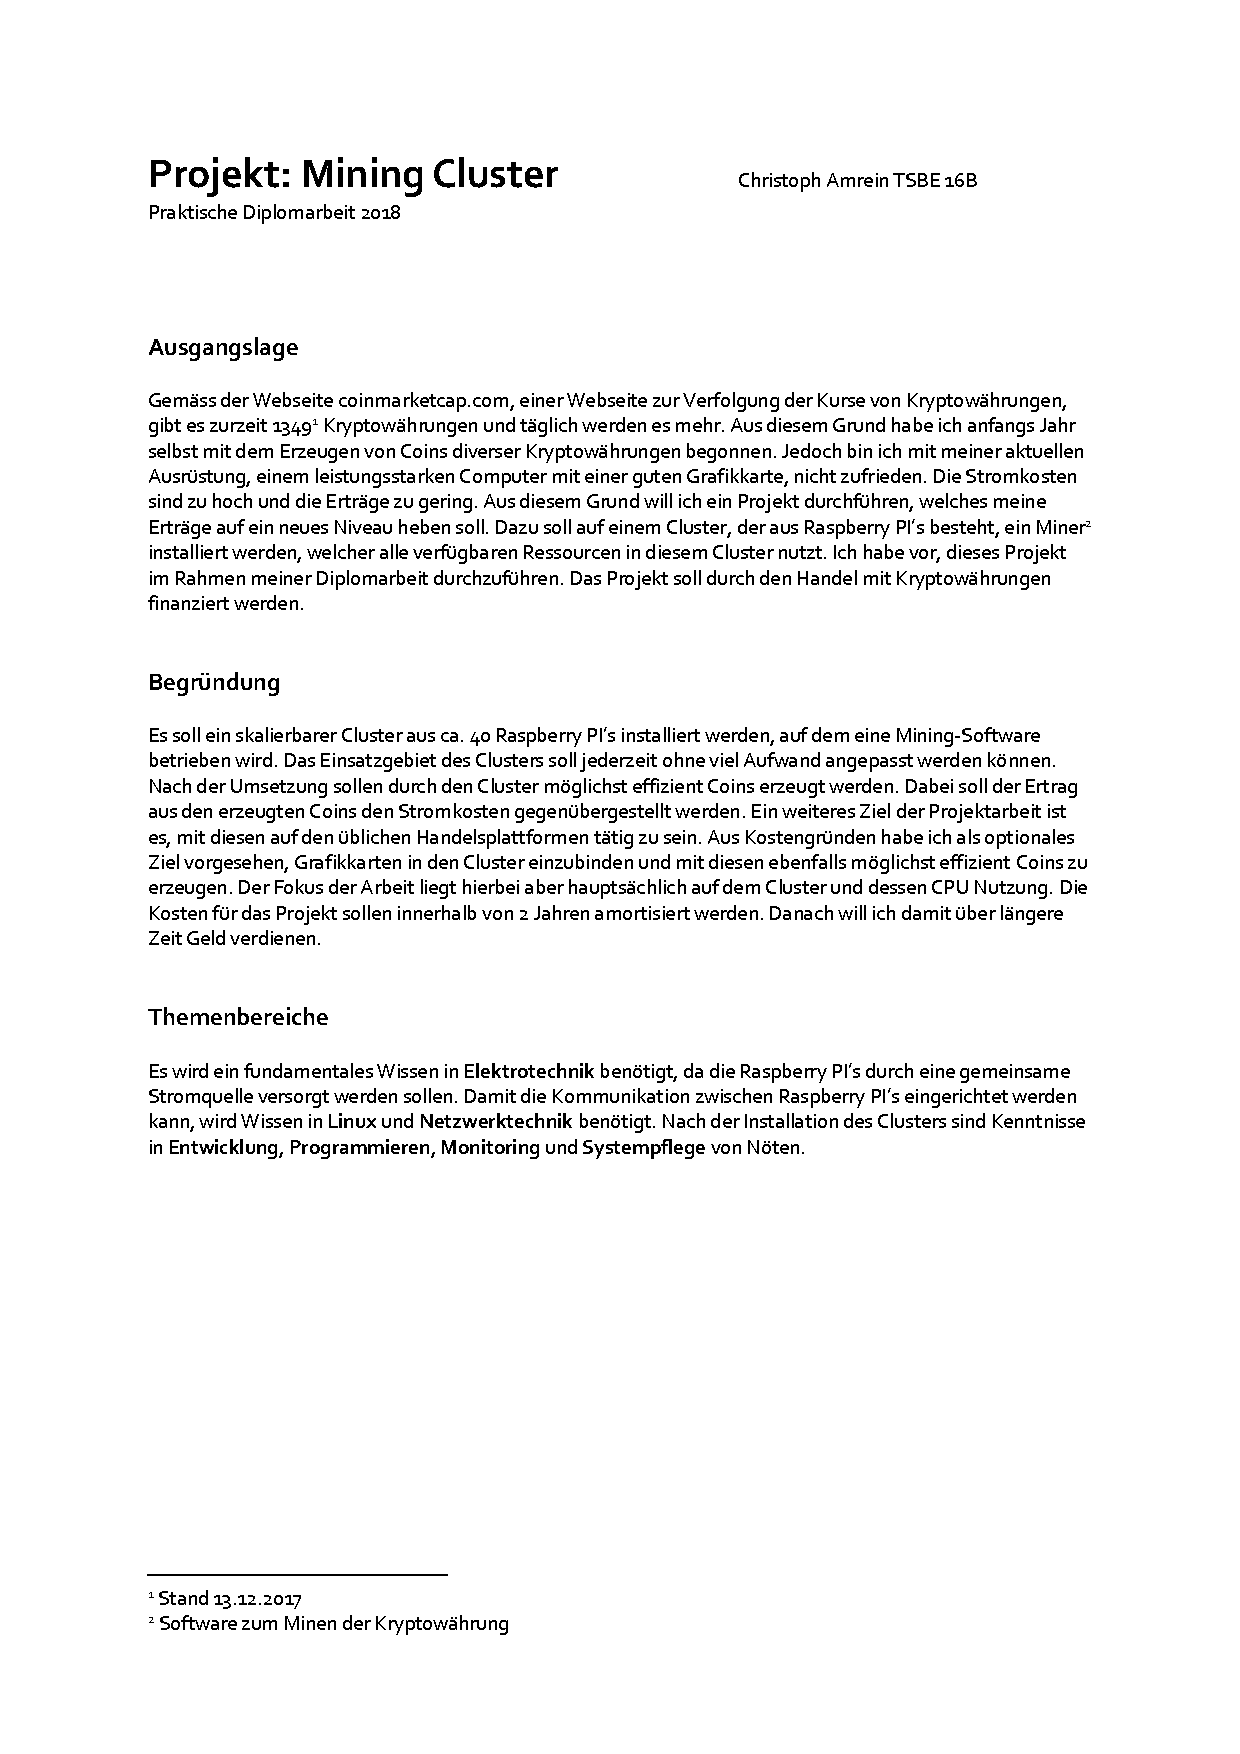
\includepdf[pages=1,scale=.8,pagecommand={\section{Diplomeingabe}\label{pdf:Diplomeingabe}},linktodoc=true]{Anhang/Diplomarbeit_Eingabe.pdf}
\includepdf[pages={2,3},scale=0.9,pagecommand={},linktodoc=true]{Anhang/Diplomarbeit_Eingabe.pdf}
\section{Testprotokoll}
% !TEX root = ../Diplombericht.tex
\subsection{Testobjekte}
\begin{table}[H]
\centering
\begin{tabular}{p{1cm}p{3cm}p{3cm}p{4cm}p{4cm}}
\hline
\rowcolor{heading} \textbf{Nr.} & \textbf{Objekt} & \textbf{Hostname} & \textbf{IP} & \textbf{MAC} \\\hline
1 & Managementnode & nebula & 192.168.1.11 & B8:27:EB:32:39:A7\\\hline
2 & Computenode 1 & c1 & 192.168.1.11 & B8:27:EB:32:39:A7\\\hline
3 & Computenode 2 & c2 & 192.168.1.12 & B8:27:EB:2E:A3:D1\\\hline
4 & Computenode 3 & c3 & 192.168.1.13 & B8:27:EB:50:45:3F\\\hline
5 & Computenode 4 & c4 & 192.168.1.14 & B8:27:EB:0D:E6:25\\\hline
6 & Computenode 5 & c5 & 192.168.1.15 & B8:27:EB:3E:96:B5\\\hline
7 & Computenode 6 & c6 & 192.168.1.16 & B8:27:EB:EE:77:DA\\\hline
8 & Computenode 7 & c7 & 192.168.1.17 & B8:27:EB:21:63:E6\\\hline
9 & Computenode 8 & c8 & 192.168.1.18 & B8:27:EB:2E:2E:CC\\\hline
10 & Computenode 9 & c9 & 192.168.1.19 & B8:27:EB:17:32:96\\\hline
11 & Computenode 10 & c10 & 192.168.1.20 & B8:27:EB:B2:1C:A9\\\hline
12 & Computenode 11 & c11 & 192.168.1.21 & B8:27:EB:AF:63:1F\\\hline
13 & Computenode 12 & c12 & 192.168.1.22 & B8:27:EB:43:00:2C\\\hline
14 & Computenode 13 & c13 & 192.168.1.23 & B8:27:EB:13:7B:18\\\hline
15 & Computenode 14 & c14 & 192.168.1.24 & B8:27:EB:43:CD:29\\\hline
16 & Computenode 15 & c15 & 192.168.1.25 & B8:27:EB:FF:C7:56\\\hline
17 & Computenode 16 & c16 & 192.168.1.26 & B8:27:EB:CE:98:66\\\hline
18 & Computenode 17 & c17 & 192.168.1.27 & B8:27:EB:5D:63:34\\\hline
19 & Computenode 18 & c18 & 192.168.1.28 & B8:27:EB:91:3E:0F\\\hline
20 & Computenode 19 & c19 & 192.168.1.29 & B8:27:EB:F4:65:EC\\\hline
21 & Computenode 20 & c20 & 192.168.1.30 & B8:27:EB:3E:AB:DC\\\hline
22 & Computenode 21 & c21 & 192.168.1.31 & B8:27:EB:66:60:F6\\\hline
23 & Computenode 22 & c22 & 192.168.1.32 & B8:27:EB:37:3F:74\\\hline
24 & Computenode 23 & c23 & 192.168.1.33 & B8:27:EB:18:5E:F0\\\hline
25 & Computenode 24 & c24 & 192.168.1.34 & B8:27:EB:B0:23:B8\\\hline
26 & Computenode 25 & c25 & 192.168.1.35 & B8:27:EB:BE:C4:94\\\hline
27 & Computenode 26 & c26 & 192.168.1.36 & B8:27:EB:FB:FF:57\\\hline
28 & Computenode 27 & c27 & 192.168.1.37 & B8:27:EB:4E:EC:CE\\\hline
29 & Computenode 28 & c28 & 192.168.1.38 & B8:27:EB:43:1C:35\\\hline
30 & Computenode 29 & c29 & 192.168.1.39 & B8:27:EB:DC:74:5F\\\hline
31 & Computenode 30 & c30 & 192.168.1.40 & B8:27:EB:D1:DE:2F\\\hline
32 & Computenode 31 & c31 & 192.168.1.41 & B8:27:EB:5E:90:34\\\hline
33 & Computenode 32 & c32 & 192.168.1.42 & B8:27:EB:DE:80:24\\\hline
34 & Computenode 33 & c33 & 192.168.1.43 & B8:27:EB:A4:79:6F\\\hline
35 & Computenode 34 & c34 & 192.168.1.44 & B8:27:EB:0A:4D:C7\\\hline
36 & Computenode 35 & c35 & 192.168.1.45 & B8:27:EB:5C:53:5F\\\hline
37 & Computenode 36 & c36 & 192.168.1.46 & B8:27:EB:F7:AF:C2\\\hline
38 & Computenode 37 & c37 & 192.168.1.47 & B8:27:EB:CE:BA:ED\\\hline
39 & Computenode 38 & c38 & 192.168.1.48 & B8:27:EB:59:38:3C\\\hline
40 & Computenode 39 & c39 & 192.168.1.49 & B8:27:EB:99:BB:8E\\\hline
41 & Computenode 40 & c40 & 192.168.1.50 & B8:27:EB:8F:7A:0D\\\hline
42 & Reservenode 1 & c41 & 192.168.1.51 & B8:27:EB:DE:C9:69\\\hline
43 & Reservenode 2 & c42 & 192.168.1.52 & B8:27:EB:7E:6F:48\\\hline
44 & Reservenode 3 & c43 & 192.168.1.53 & B8:27:EB:5D:DD:FE\\\hline
45 & Reservenode 4 & c44 & 192.168.1.54 & B8:27:EB:A6:6D:4D\\\hline
46 & Reservenode 5 & c45 & 192.168.1.55 & B8:27:EB:0C:63:10\\\hline
\end{tabular}
\caption{Computenode Namen}
\end{table}

\subsection{Arbeitsjournal}
\label{app:Arbeitsjournal}

\tabelleAnhang{Arbeitsjournal}

\subsection{Protkolle}
\label{app:Protokolle}


%\subsection{Detaillierte Zeitplanung}
%\label{app:Zeitplanung}

%\tabelleAnhang{ZeitplanungKomplett}

%\subsection{Lastenheft (Auszug)}
\label{app:Lastenheft}
Es folgt ein Auszug aus dem Lastenheft mit Fokus auf die Anforderungen:

Die Anwendung muss folgende Anforderungen erfüllen: 
\begin{enumerate}[itemsep=0em,partopsep=0em,parsep=0em,topsep=0em]
\item Verarbeitung der Moduldaten
	\begin{enumerate}
	\item Die Anwendung muss die von Subversion und einem externen Programm bereitgestellten Informationen (z.B. Source-Benutzer, -Datum, Hash) verarbeiten.
	\item Auslesen der Beschreibung und der Stichwörter aus dem Sourcecode.
	\end{enumerate}
\item Darstellung der Daten
	\begin{enumerate}
	\item Die Anwendung muss eine Liste aller Module erzeugen inkl. Source-Benutzer und -Datum, letztem Commit-Benutzer und -Datum für alle drei Umgebungen. 
	\item Verknüpfen der Module mit externen Tools wie z.B. Wiki-Einträgen zu den Modulen oder dem Sourcecode in Subversion.
	\item Die Sourcen der Umgebungen müssen verglichen und eine schnelle Übersicht zur Einhaltung des allgemeinen Entwicklungsprozesses gegeben werden. 
	\item Dieser Vergleich muss auf die von einem bestimmten Benutzer bearbeiteten Module eingeschränkt werden können. 
	\item Die Anwendung muss in dieser Liste auch Module anzeigen, die nach einer Bearbeitung durch den gesuchten Benutzer durch jemand anderen bearbeitet wurden. 
	\item Abweichungen sollen kenntlich gemacht werden. 
	\item Anzeigen einer Übersichtsseite für ein Modul mit allen relevanten Informationen zu diesem.
	\end{enumerate}
\item Sonstige Anforderungen
	\begin{enumerate}
	\item Die Anwendung muss ohne das Installieren einer zusätzlichen Software über einen Webbrowser im Intranet erreichbar sein.
	\item Die Daten der Anwendung müssen jede Nacht \bzw nach jedem \acs{SVN}-Commit automatisch aktualisiert werden. 
	\item Es muss ermittelt werden, ob Änderungen auf der Produktionsumgebung vorgenommen wurden, die nicht von einer anderen Umgebung kopiert wurden. Diese Modulliste soll als Mahnung per E-Mail an alle Entwickler geschickt werden (Peer Pressure).
	\item Die Anwendung soll jederzeit erreichbar sein.
	\item Da sich die Entwickler auf die Anwendung verlassen, muss diese korrekte Daten liefern und darf keinen Interpretationsspielraum lassen.
	\item Die Anwendung muss so flexibel sein, dass sie bei Änderungen im Entwicklungsprozess einfach angepasst werden kann.
	\end{enumerate}
\end{enumerate}


\clearpage

%\subsection{Use Case-Diagramm}
%\label{app:UseCase}
%Use Case-Diagramme und weitere \acs{UML}-Diagramme kann man auch direkt mit \LaTeX{} zeichnen, siehe \zB %%%%%\url{http://metauml.sourceforge.net/old/usecase-diagram.html}.
%\begin{figure}[htb]
%\centering
%\includegraphicsKeepAspectRatio{UseCase.pdf}{0.7}
%\caption{Use Case-Diagramm}
%\end{figure}

%\subsection{Pflichtenheft (Auszug)}
\label{app:Pflichtenheft}

\subsubsection*{Zielbestimmung}

\begin{enumerate}[itemsep=0em,partopsep=0em,parsep=0em,topsep=0em]
\item Musskriterien % Wikipedia: für das Produkt unabdingbare Leistungen, die in jedem Fall erfüllt werden müssen
	\begin{enumerate}
	\item Modul-Liste: Zeigt eine filterbare Liste der Module mit den dazugehörigen Kerninformationen sowie Symbolen zur Einhaltung des Entwicklungsprozesses an
		\begin{itemize}
		\item In der Liste wird der Name, die Bibliothek und Daten zum Source und Kompilat eines Moduls angezeigt.
		\item Ebenfalls wird der Status des Moduls hinsichtlich Source und Kompilat angezeigt. Dazu gibt es unterschiedliche Status-Zeichen, welche symbolisieren in wie weit der Entwicklungsprozess eingehalten wurde \bzw welche Schritte als nächstes getan werden müssen. So gibt es \zB Zeichen für das Einhalten oder Verletzen des Prozesses oder den Hinweis auf den nächsten zu tätigenden Schritt. 
		\item Weiterhin werden die Benutzer und Zeitpunkte der aktuellen Version der Sourcen und Kompilate angezeigt. Dazu kann vorher ausgewählt werden, von welcher Umgebung diese Daten gelesen werden sollen. 
		\item Es kann eine Filterung nach allen angezeigten Daten vorgenommen werden. Die Daten zu den Sourcen sind historisiert. Durch die Filterung ist es möglich, auch Module zu finden, die in der Zwischenzeit schon von einem anderen Benutzer editiert wurden.
		\end{itemize}
	\item Tag-Liste: Bietet die Möglichkeit die Module anhand von Tags zu filtern. 
		\begin{itemize}
		\item Es sollen die Tags angezeigt werden, nach denen bereits gefiltert wird und die, die noch der Filterung hinzugefügt werden könnten, ohne dass die Ergebnisliste leer wird.
		\item Zusätzlich sollen die Module angezeigt werden, die den Filterkriterien entsprechen. Sollten die Filterkriterien leer sein, werden nur die Module angezeigt, welche mit einem Tag versehen sind.
		\end{itemize}
	\item Import der Moduldaten aus einer bereitgestellten \acs{CSV}-Datei
		\begin{itemize}
		\item Es wird täglich eine Datei mit den Daten der aktuellen Module erstellt. Diese Datei wird (durch einen Cronjob) automatisch nachts importiert.
		\item Dabei wird für jedes importierte Modul ein Zeitstempel aktualisiert, damit festgestellt werden kann, wenn ein Modul gelöscht wurde.
		\item Die Datei enthält die Namen der Umgebung, der Bibliothek und des Moduls, den Programmtyp, den Benutzer und Zeitpunkt des Sourcecodes sowie des Kompilats und den Hash des Sourcecodes.
		\item Sollte sich ein Modul verändert haben, werden die entsprechenden Daten in der Datenbank aktualisiert. Die Veränderungen am Source werden dabei aber nicht ersetzt, sondern historisiert.
		\end{itemize}
	\item Import der Informationen aus \ac{SVN}. Durch einen \gqq{post-commit-hook} wird nach jedem Einchecken eines Moduls ein \acs{PHP}-Script auf der Konsole aufgerufen, welches die Informationen, die vom \ac{SVN}-Kommandozeilentool geliefert werden, an \acs{NatInfo} übergibt.
	\item Parsen der Sourcen
		\begin{itemize}
		\item Die Sourcen der Entwicklungsumgebung werden nach Tags, Links zu Artikeln im Wiki und Programmbeschreibungen durchsucht.
		\item Diese Daten werden dann entsprechend angelegt, aktualisiert oder nicht mehr gesetzte Tags/Wikiartikel entfernt.
		\end{itemize}
	\item Sonstiges
		\begin{itemize}
		\item Das Programm läuft als Webanwendung im Intranet.
		\item Die Anwendung soll möglichst leicht erweiterbar sein und auch von anderen Entwicklungsprozessen ausgehen können.
		\item Eine Konfiguration soll möglichst in zentralen Konfigurationsdateien erfolgen.
		\end{itemize}
	\end{enumerate}
\end{enumerate}

\subsubsection*{Produkteinsatz}

\begin{enumerate}[itemsep=0em,partopsep=0em,parsep=0em,topsep=0em]
\item{Anwendungsbereiche\\
Die Webanwendung dient als Anlaufstelle für die Entwicklung. Dort sind alle Informationen für die Module an einer Stelle gesammelt. Vorher getrennte Anwendungen werden ersetzt \bzw verlinkt.}
\item{Zielgruppen\\
\NI wird lediglich von den \ac{Natural}-Entwicklern in der EDV-Abteilung genutzt.}
\item{Betriebsbedingungen\\ % Wikipedia: physikalische Umgebung des Systems, tägliche Betriebszeit, ständige Beobachtung des Systems durch Bediener oder unbeaufsichtigter Betrieb
Die nötigen Betriebsbedingungen, also der Webserver, die Datenbank, die Versionsverwaltung, das Wiki und der nächtliche Export sind bereits vorhanden und konfiguriert. Durch einen täglichen Cronjob werden entsprechende Daten aktualisiert, die Webanwendung ist jederzeit aus dem Intranet heraus erreichbar.}
\end{enumerate}


%\subsection{Datenbankmodell}
%\label{app:Datenbankmodell}
%ER-Modelle kann man auch direkt mit \LaTeX{} zeichnen, siehe \zB \url{http://www.texample.net/tikz/examples/entity-relationship-diagram/}.
%\begin{figure}[htb]
%\centering
%\includegraphicsKeepAspectRatio{database.pdf}{1}
%\caption{Datenbankmodell}
%\end{figure}
%\clearpage

%\subsection{Oberflächenentwürfe}
\label{app:Entwuerfe}
\begin{figure}[htb]
\centering
\includegraphicsKeepAspectRatio{MockupModules.pdf}{0.7}
\caption{Liste der Module mit Filtermöglichkeiten}
\end{figure}

\begin{figure}[htb]
\centering
\includegraphicsKeepAspectRatio{MockupModul.pdf}{0.7}
\caption{Anzeige der Übersichtsseite einzelner Module}
\end{figure}

\begin{figure}[htb]
\centering
\includegraphicsKeepAspectRatio{MockupTag.pdf}{0.7}
\caption{Anzeige und Filterung der Module nach Tags}
\end{figure}

%\clearpage
%\subsection{Screenshots der Anwendung}
\label{Screenshots}
\begin{figure}[htb]
\centering
\includegraphicsKeepAspectRatio{tagliste.pdf}{1}
\caption{Anzeige und Filterung der Module nach Tags}
\end{figure}
\clearpage
\begin{figure}[htb]
\centering
\includegraphicsKeepAspectRatio{modulliste.pdf}{1}
\caption{Liste der Module mit Filtermöglichkeiten}
\end{figure}
\clearpage

%\subsection{Entwicklerdokumentation}
\label{app:Doc}
\begin{center}
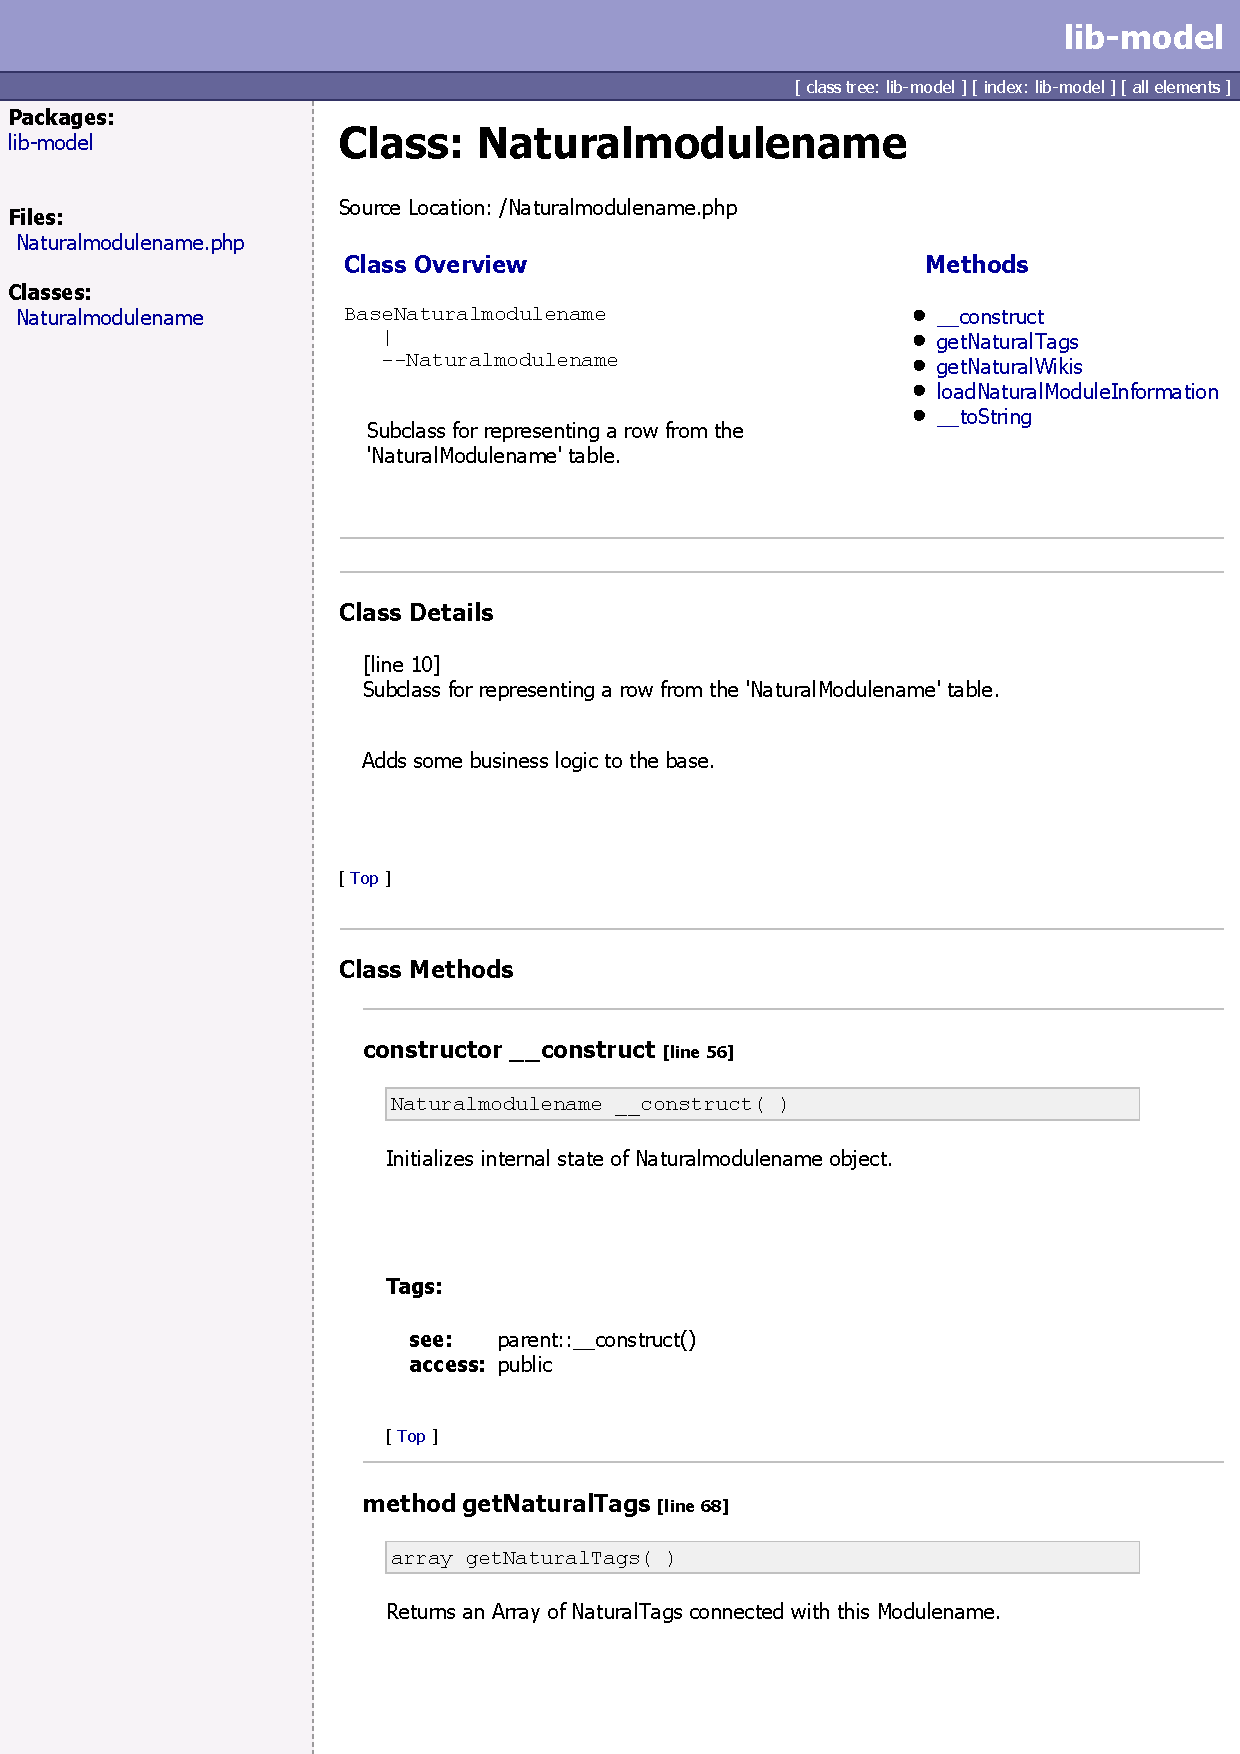
\includegraphics[page=1, width=0.9\textwidth]{doc.pdf}

\includegraphics[page=2, width=0.9\textwidth]{doc.pdf}
\end{center}

%\clearpage
%\subsection{Testfall und sein Aufruf auf der Konsole}
\label{app:Test}
\lstinputlisting[language=php, caption={Testfall in PHP}]{Listings/tests.php}
\clearpage
\begin{figure}[htb]
\centering
\includegraphicsKeepAspectRatio{testcase.jpg}{1}
\caption{Aufruf des Testfalls auf der Konsole}
\end{figure}


%\subsection{Klasse: ComparedNaturalModuleInformation}
%\label{app:CNMI}
%Kommentare und simple Getter/Setter werden nicht angezeigt.
%\lstinputlisting[language=php, caption={Klasse: ComparedNaturalModuleInformation}]{Listings/cnmi.php}
%\clearpage

%\subsection{Klassendiagramm}
%\label{app:Klassendiagramm}
%Klassendiagramme und weitere \acs{UML}-Diagramme kann man auch direkt mit \LaTeX{} zeichnen, siehe \zB %\url{http://metauml.sourceforge.net/old/class-diagram.html}.
%\begin{figure}[htb]
%\centering
%\includegraphicsKeepAspectRatio{Klassendiagramm.pdf}{1}
%\caption{Klassendiagramm}
%\end{figure}
%\clearpage

\subsection{Datenblätter}
\label{app:Datenblätter}

\subsection{Produktinformationen}
\label{app:Produktinformationen}


\subsection{Benutzerdokumentation}
\label{app:BenutzerDoku}
Ausschnitt aus der Benutzerdokumentation:

\begin{table}[htb]
\begin{tabularx}{\textwidth}{cXX}
\rowcolor{heading}\textbf{Symbol} & \textbf{Bedeutung global} & \textbf{Bedeutung einzeln} \\
\includegraphicstotab[]{weather-clear.png} & Alle Module weisen den gleichen Stand auf. & Das Modul ist auf dem gleichen Stand wie das Modul auf der vorherigen Umgebung. \\
\rowcolor{odd}\includegraphicstotab[]{weather-clear-night.png} & Es existieren keine Module (fachlich nicht möglich). & Weder auf der aktuellen noch auf der vorherigen Umgebung sind Module angelegt. Es kann also auch nichts übertragen werden. \\
\includegraphicstotab[]{weather-few-clouds-night.png} & Ein Modul muss durch das Übertragen von der vorherigen Umgebung erstellt werden. & Das Modul der vorherigen Umgebung kann übertragen werden, auf dieser Umgebung ist noch kein Modul vorhanden. \\
\rowcolor{odd}\includegraphicstotab[]{weather-few-clouds.png} & Auf einer vorherigen Umgebung gibt es ein Modul, welches übertragen werden kann, um das nächste zu aktualisieren. & Das Modul der vorherigen Umgebung kann übertragen werden um dieses zu aktualisieren. \\
\includegraphicstotab[]{weather-storm.png} & Ein Modul auf einer Umgebung wurde entgegen des Entwicklungsprozesses gespeichert. & Das aktuelle Modul ist neuer als das Modul auf der vorherigen Umgebung oder die vorherige Umgebung wurde übersprungen. \\
\end{tabularx}
\end{table}


